
\makesection{Motivación}


\begin{frame}{Evolución de la Violencia en Colombia}
    \begin{figure}[ht]
        \centering
        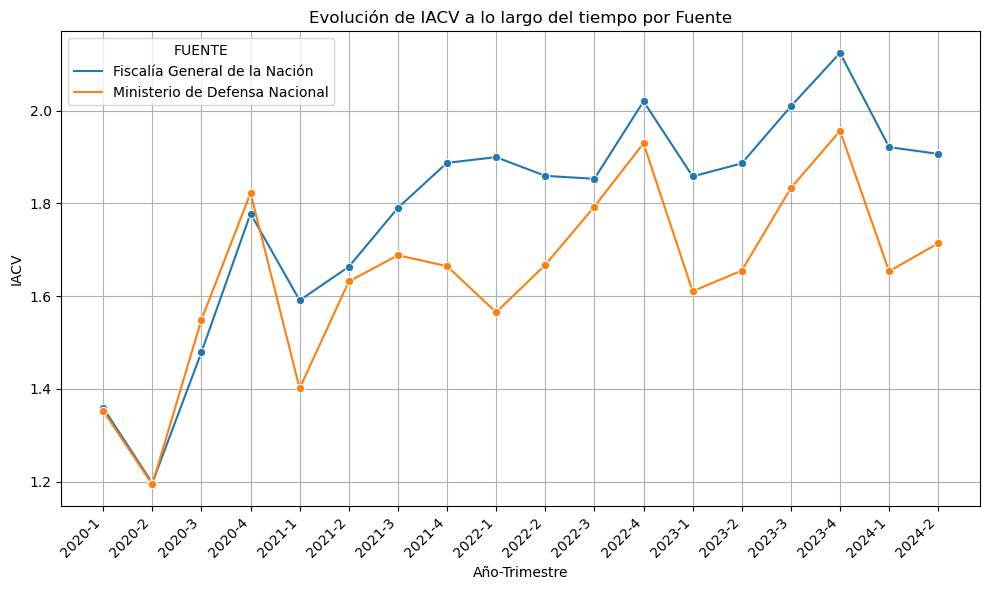
\includegraphics[width=0.9\textwidth, height=0.7\textheight, keepaspectratio]{images/image 7.png}
    \end{figure}
    \centering
    \footnotesize\textit{Fuente: Datos  MinDefensa. Elaboración propia}
\end{frame}

\begin{frame}{Vulnerabilidad municipal a la violencia}
    \begin{columns}[T]
        % Columna izquierda
        \begin{column}{0.48\textwidth}
            \centering
            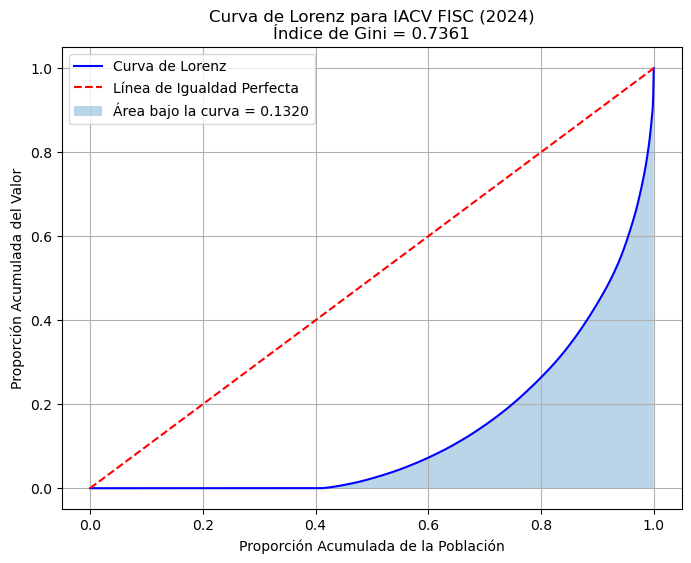
\includegraphics[width=\textwidth, height=0.65\textheight, keepaspectratio]{images/image 4.png}
        \end{column}
        
        % Columna derecha
        \begin{column}{0.48\textwidth}
            \centering
            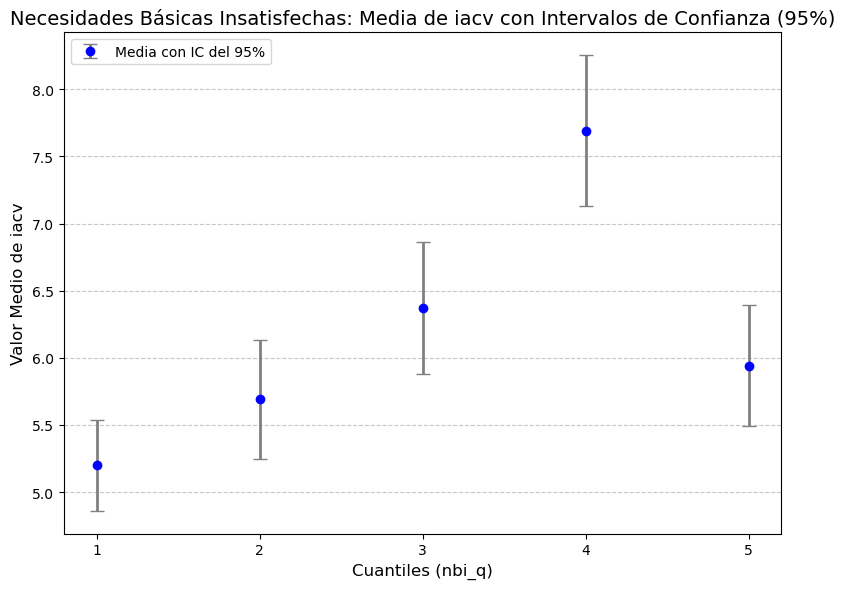
\includegraphics[width=\textwidth, height=0.65\textheight, keepaspectratio]{images/output1.png}
        \end{column}
    \end{columns}
    \vspace{0.2cm}
    \centering
    \footnotesize\textit{Fuente: Datos Panel CEDE y MinDefensa. Elaboración propia}
\end{frame}



\begin{frame}{Motivación}
    \small
    \begin{block}{¿Por qué importa esta pregunta?}
        \begin{itemize}
            \item La violencia atípica tiene \textbf{alto impacto social} y \textbf{poca capacidad de respuesta}.
            \item Las herramientas actuales (SAT) son cualitativas y pueden no detectar patrones emergentes.
        \end{itemize}
    \end{block}
    
    \begin{block}{¿Qué propone esta tesis?}
        \begin{itemize}
            \item Usar \textbf{aprendizaje automático} para predecir eventos críticos.
            \item Complementar el SAT con una herramienta cuantitativa y replicable.
        \end{itemize}
    \end{block}

%    \begin{block}{¿Por qué ahora?}
%        \begin{itemize}
%            \item Mayor disponibilidad de datos detallados sobre violencia y contexto municipal.
%            \item Necesidad urgente de mejorar la prevención frente a conflictos armados y crimen organizado.
%        \end{itemize}
%    \end{block}
\end{frame}

%\begin{frame}{Motivación}
%    \small
%    \begin{itemize}
%        \item La violencia atípica genera altos costos sociales, económicos y humanitarios, especialmente cuando se presenta de forma repentina e intensa, dejando poco tiempo de respuesta institucional.
        
%        \vspace{0.35cm}
%        \item El Sistema de Alertas Tempranas (SAT) ha sido clave para prevenir violaciones a los derechos humanos, pero se basa en metodologías cualitativas que pueden no ser tan rápidas, ni tomar en cuenta patrones no observables.
        
%        \vspace{0.35cm}
%        \item Integrar herramientas de aprendizaje automático permite \textbf{identificar con anticipación eventos atípicos de violencia} apoyando la capacidad de reacción del Estado.
        
%        \vspace{0.35cm}
%        \item Esta tesis busca ofrecer una herramienta cuantitativa que complemente el SAT y \textbf{fortalezca la prevención basada en evidencia}.
%    \end{itemize}
%\end{frame}